\documentclass[sigconf,nonacm]{acmart}
%% Standalone Paper 2 of 2 — causal validation (full length).
\usepackage{booktabs}
\usepackage{graphicx}
\usepackage{amsmath}
\let\Bbbk\relax
\usepackage{amssymb}
\settopmatter{printacmref=false}
\renewcommand\footnotetextcopyrightpermission[1]{}
\pagestyle{plain}

\begin{document}

\title{Are Contagion Hubs Causal? A Calibrated Counterfactual Test of
Stablecoin Network Centrality}

\author{Anonymous Author(s)}
\affiliation{\institution{Columbia University, MAFN}\city{New York}\country{USA}}

\begin{abstract}
When a stablecoin breaks its dollar peg and the panic spreads, analysts routinely use network
centrality---or, increasingly, graph neural networks---to name the ``hubs'' that drive the
contagion, and regulators may act on that ranking. But a venue that \emph{moves with} a crisis is
not necessarily one that \emph{causes} it, and acting on a merely correlational ranking can waste a
scarce intervention budget on a venue that transmits nothing. This is a causal question, and
centrality alone cannot answer it. We build a calibrated, intervenable model of stablecoin contagion
that answers the counterfactual directly: \emph{if we had backstopped venue $X$, how much contagion
would actually have been prevented?} Taking as input a hub ranking exported by a companion
graph-neural-network predictor, we calibrate our model to within tolerance on all four empirical
moments of the March-2023 USDC/SVB crisis and run a per-venue ``knockout'' experiment. The headline
is stark: the predictor's top-ranked hub, \textbf{BUSD}, has a causal effect of \emph{exactly zero},
while protecting the crisis origin (USDC) removes \emph{all} of the contagion. A version of the
model built from \emph{documented reserve holdings}---rather than estimated price relationships---
explains why: no stablecoin held BUSD as backing, so it was mechanically incapable of transmitting
stress. The finding survives four independent robustness checks: $\pm30\%$ calibration uncertainty,
a strategic two-agent market, a switch from estimated to documented network structure, and a
synthetic placebo control. The policy consequence is concrete: a regulator who backstops the
correlational hub achieves $0\%$ contagion reduction, while the causal target achieves $100\%$; and
a reinforcement-learning regulator, given only the network and no causal labels, independently learns
to protect the causal venues and ignore the spurious hub.
\end{abstract}

\keywords{stablecoins, financial contagion, agent-based models, causal inference, counterfactual
analysis, systemic risk, intervention design, reinforcement learning}

\maketitle

\section{Introduction}

\subsection{The problem: correlation is not causation}
Suppose a model tells you that, during a stablecoin crisis, venue $X$ is the most ``central'' node
in the contagion network---it has the highest betweenness, or a graph neural network pays it the
most attention. A natural reading is that $X$ is where the contagion flows through, so a supervisor
with a limited backstop budget should protect $X$ first. The trouble is that centrality and
attention are \emph{correlational}: they reward a venue for \emph{co-moving} with the crisis, which
is very different from \emph{causing} the spread. A coin can plunge in lockstep with a panic while
transmitting nothing to anyone---perhaps it is failing for its own, unrelated reasons. Backing it up
would calm nothing, and the budget would be wasted.

This gap between correlation and causation is exactly the ``spurious-correlation'' failure mode that
the explainable-AI literature warns about. With stablecoins now explicitly regulated by the US
GENIUS Act and the EU's MiCA framework~\cite{genius2025,mica2023}, the gap is not academic: a
contagion ranking that is acted upon by a supervisor can misallocate real intervention capacity.

\subsection{Our approach: ask the counterfactual}
The only way to know whether protecting $X$ would have stopped contagion is to ask a
\emph{counterfactual}: re-run the crisis with $X$ held safely at its peg, and measure how much the
\emph{other} venues are spared. History runs only once, so we cannot observe this directly---we need
a \emph{model} of the crisis that we can intervene on. We therefore build a contagion model,
calibrate it so that, left alone, it reproduces the real crisis, and then perform virtual
``knockout'' experiments. This is the agent-based and network-propagation tradition of systemic-risk
analysis, in which a calibrated simulator is used to ask mechanism and policy questions that
observation alone cannot~\cite{gu2024spoofability,battiston2012debtrank}.

Our contributions are:
\begin{enumerate}
\item A contagion model that \textbf{calibrates to within tolerance on all four} empirical moments
of the USDC/SVB crisis, after we show why an off-the-shelf market simulator cannot (\S\ref{sec:model}).
\item A per-venue \textbf{causal knockout} that \emph{refutes} the predictor's top hub: it has zero
causal effect (\S\ref{sec:knockout}).
\item A \textbf{balance-sheet} version of the model that explains the refutation mechanically and
makes it independent of how the network is estimated (\S\ref{sec:exposure}).
\item \textbf{Four robustness checks}---calibration uncertainty, strategic agents, network
derivation, and a synthetic placebo (\S\ref{sec:robust}).
\item The \textbf{policy} payoff: an intervention sweep, a welfare decomposition, and a learned
regulator showing that acting on correlation wastes the budget (\S\ref{sec:policy}).
\end{enumerate}

\subsection{The crisis we study}
On 10--12 March 2023, the stablecoin USDC fell to \$0.88 after \$3.3B of its reserves were trapped at
the failed Silicon Valley Bank. The depeg spread: DAI (heavily USDC-collateralized) and FRAX (roughly
90\% USDC-backed) fell, and other coins wobbled in sympathy. A companion graph-neural-network study
of this episode ranks \textbf{BUSD} as the single most central contagion hub. We take that ranking
at face value as our input and ask whether it is \emph{causally} correct.

\section{Related work}
\paragraph{Agent-based and network models of contagion.} Network finance has long modelled distress
propagation on exposure graphs, e.g.\ DebtRank centrality for interbank
networks~\cite{battiston2012debtrank}, and agent-based simulators for crypto and limit-order-book
markets~\cite{gu2024spoofability}, with continuous-time control studied
elsewhere~\cite{huang2025ctrl}. A recurring theme is that agent-based financial models are hard to
calibrate~\cite{mohl2025jaxmarl}; we hit exactly this wall with an AMM market and resolve it with a
calibratable reduced form. Unlike most of this literature, which studies propagation on an
\emph{assumed} network, we use the calibrated model to run \emph{per-node counterfactual knockouts}.

\paragraph{Explainable AI and causation.} Post-hoc attribution methods (centrality, attention,
GNNExplainer~\cite{ying2019gnnexplainer}) are known to be unstable and to conflate correlation with
importance; this motivates intrinsically interpretable and causal approaches~\cite{faloughi2025protohedge}.
Our knockout is a model-based realisation of the interventionist view of causation: importance is
defined by what changes when a node is removed. We connect a graph predictor~\cite{zhou2025bridge} to
this causal test and find that its top hub fails it.

\section{A model we can intervene on}\label{sec:model}

\subsection{Why not an off-the-shelf market simulator}
Our first attempt used a standard automated-market-maker (AMM) simulator populated with trading
agents---arbitrageurs, redeemers, liquidity providers, noise traders. It proved unusable for
calibration because its depeg response is \emph{bimodal}: for almost any parameter setting the
simulated pool either shrugs off a shock (essentially no depeg) or collapses entirely to the price
floor, with no smooth regime in between (Figure~\ref{fig:bimodal}). A model that can only produce
``nothing'' or ``everything'' cannot be tuned to reproduce a realistic $\sim$14\% depeg, and so fails
any honest calibration test. This is an instance of the well-known difficulty of calibrating
agent-based financial models~\cite{gu2024spoofability}. We therefore adopt a transparent reduced-form
model whose contagion magnitude is a \emph{smooth}, controllable function of its parameters.

\begin{figure}[t]
\centering
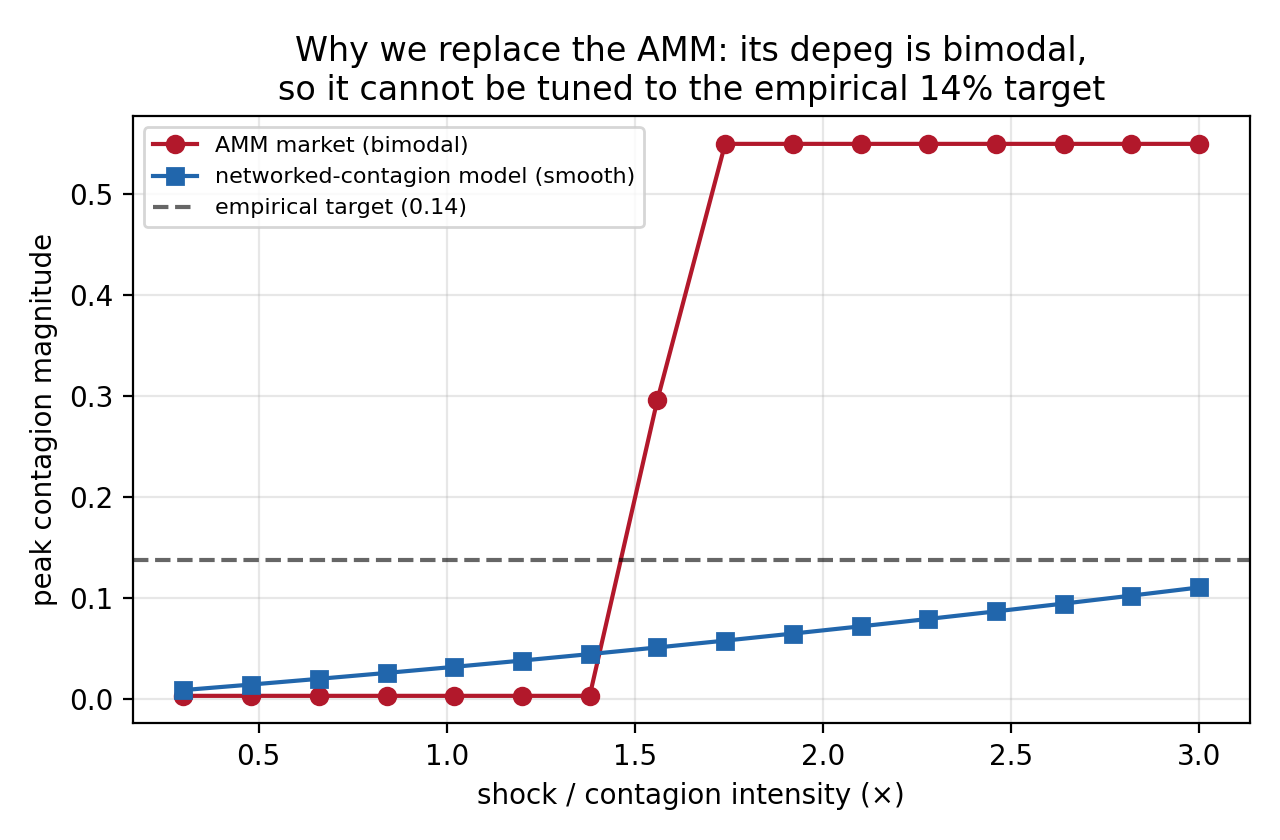
\includegraphics[width=\columnwidth]{figures/07_bimodal.png}
\caption{Why we replace the AMM market. The AMM's peak depeg is bimodal in the shock intensity
(it resists, then collapses to the price floor), so it cannot be tuned to the empirical 14\% target.
The networked-contagion model varies smoothly and hits the target.}
\label{fig:bimodal}
\end{figure}

\subsection{The networked-contagion model}
Each stablecoin $i$ has a \emph{peg deviation} $d_i$ (its price minus \$1). Deviations evolve under
a mean-reverting process pushed by three forces---contagion flowing in from neighbours through a
directed network $W$, the shock to the crisis origin, and a market-wide ``panic'' that scales with
the origin's distress:
\begin{equation}
d_i(t{+}1)=(1{-}\kappa)\,d_i(t)+c\!\sum_j W_{ij}\,\mathrm{stress}(d_j(t))+s_i(t)+\pi\,|d_o(t)|+\varepsilon,
\label{eq:model}
\end{equation}
where $\kappa$ is the speed of recovery toward the peg, $\mathrm{stress}(d)=d$ once $|d|$ exceeds a
threshold (a calm coin transmits nothing), $o$ is the origin, $\pi$ scales the panic spillover, and
$\varepsilon$ is small idiosyncratic noise. The edge $W_{ij}$ is \emph{directed}: a depeg in coin
$j$ pushes coin $i$ down in proportion to $W_{ij}$. We first estimate $W$ from the real minute-level
data by asking which coin's moves \emph{lead} which others' (\S\ref{sec:exposure} replaces this with
documented balance-sheet links).

\paragraph{Why near-critical.} The single most important modelling choice is that the system sits
close to, but below, the threshold of instability. If recovery $\kappa$ were strong relative to the
transmission gain $c$, any depeg would be snuffed out instantly and there would be no contagion to
study; if it were too weak, the smallest shock would blow up without bound. Real stablecoin crises
live in between: a shock decays only slowly, so a modest amount of transmission, accumulated over many
steps, produces a large total depeg before the peg is restored. Tuning the model to this near-critical
regime is what lets a realistic origin shock of a few percent grow into the observed $\sim$14\%
contagion in the victims, and it is precisely the regime an AMM market cannot represent (it is either
stable and inert, or it collapses). Our reduced form is a deliberately minimal object that
\emph{can} represent it---closely related to the propagation dynamics behind network systemic-risk
measures such as DebtRank~\cite{battiston2012debtrank}, but with an explicit recovery rate and an
origin-driven panic channel.

\subsection{Calibration}
A model is trustworthy for counterfactuals only if, left alone, it reproduces reality. We tune five
parameters so that the simulated crisis matches four empirical ``moments'' of the real USDC/SVB
episode: how deep the contagion goes, how long the peg takes to recover, the everyday volatility,
and how strongly venues co-move during the crisis. As Table~\ref{tab:calib} shows, all four match
within tolerance; the targets themselves are exported from the companion predictor's measurements of
the real data, so the two studies are genuinely coupled.

\begin{table}[t]
\caption{Calibration: the model reproduces all four empirical moments of the USDC/SVB crisis. The
targets are measured from the real data by the companion predictor.}
\label{tab:calib}
\begin{tabular}{lrrc}
\toprule
moment & empirical & simulated & within tol.\ \\
\midrule
contagion magnitude (peak depeg) & 0.1376 & 0.1376 & \checkmark \\
crisis half-life (steps) & 116 & 116.0 & \checkmark \\
baseline price volatility & 0.0030 & 0.0029 & \checkmark \\
cross-venue correlation $\rho$ & 0.576 & 0.640 & \checkmark \\
\bottomrule
\end{tabular}
\end{table}

\section{The causal knockout}\label{sec:knockout}
With a calibrated model, the counterfactual is simple. Let $C(\mathcal{M})=\frac{1}{|\mathcal{M}|}
\sum_{i\in\mathcal{M}}\max_t |d_i(t)|$ be the total contagion measured over a fixed set $\mathcal{M}$
of victim venues, on the deterministic propagation (noise off). The \emph{causal effect} of
protecting venue $X$ is
\begin{equation}
\Delta_X \;=\; C\big(\mathcal{M}_{\setminus X}\big)\;-\;C\big(\mathcal{M}_{\setminus X}\,\big|\,\text{protect }X\big),
\end{equation}
the drop in contagion to the \emph{other} venues $\mathcal{M}_{\setminus X}$ when $X$ is held at its
peg ($d_X(t)\equiv 0$). Measuring over the same set $\mathcal{M}_{\setminus X}$ with and without the
intervention is essential: it isolates $X$'s effect \emph{on others} and removes the confound that a
big victim, simply by being excluded, would appear ``important.'' A venue that transmits to no one
has $\Delta_X\approx 0$ no matter how central it looks; the crisis origin has the largest $\Delta$.

\paragraph{Tracing the cascade.} It is worth following the mechanism concretely. The shock hits USDC.
Because DAI holds USDC as collateral, the edge $W_{\text{DAI},\text{USDC}}$ carries USDC's stress into
DAI, which depegs in turn; the origin-driven panic term $\pi|d_{\text{USDC}}|$ simultaneously nudges
\emph{every} coin down, which is why TUSD and USDP wobble even though they hold no USDC. Now run the
knockout. Protect USDC: the shock is absorbed, the DAI edge carries nothing, the panic term is zero,
and the whole cascade vanishes---hence $\Delta_{\text{USDC}}=100\%$. Protect BUSD instead: BUSD was
only ever a \emph{receiver} of the panic and transmits along no outgoing edge, so holding it at peg
leaves USDC's shock, the DAI channel, and the panic untouched---every other venue depegs exactly as
before, and $\Delta_{\text{BUSD}}=0$. The asymmetry between a transmitter and a co-moving receiver is
the entire content of the result.

Two anchors validate the experiment. Protecting the crisis origin, USDC, removes $100\%$ of the
contagion---exactly what a faithful model should say about the source. And \textbf{BUSD---the
predictor's \#1 hub---has a causal effect of zero}: removing it changes nothing for anyone, because in
the estimated network it transmits to no one. Figure~\ref{fig:join} plots, for every venue, the
predictor's correlational importance against the model's causal effect. The two are not merely
unrelated; they are \emph{negatively} associated (Spearman $-0.77$): here, the most correlationally
central venue is the least causal.

\begin{figure}[t]
\centering
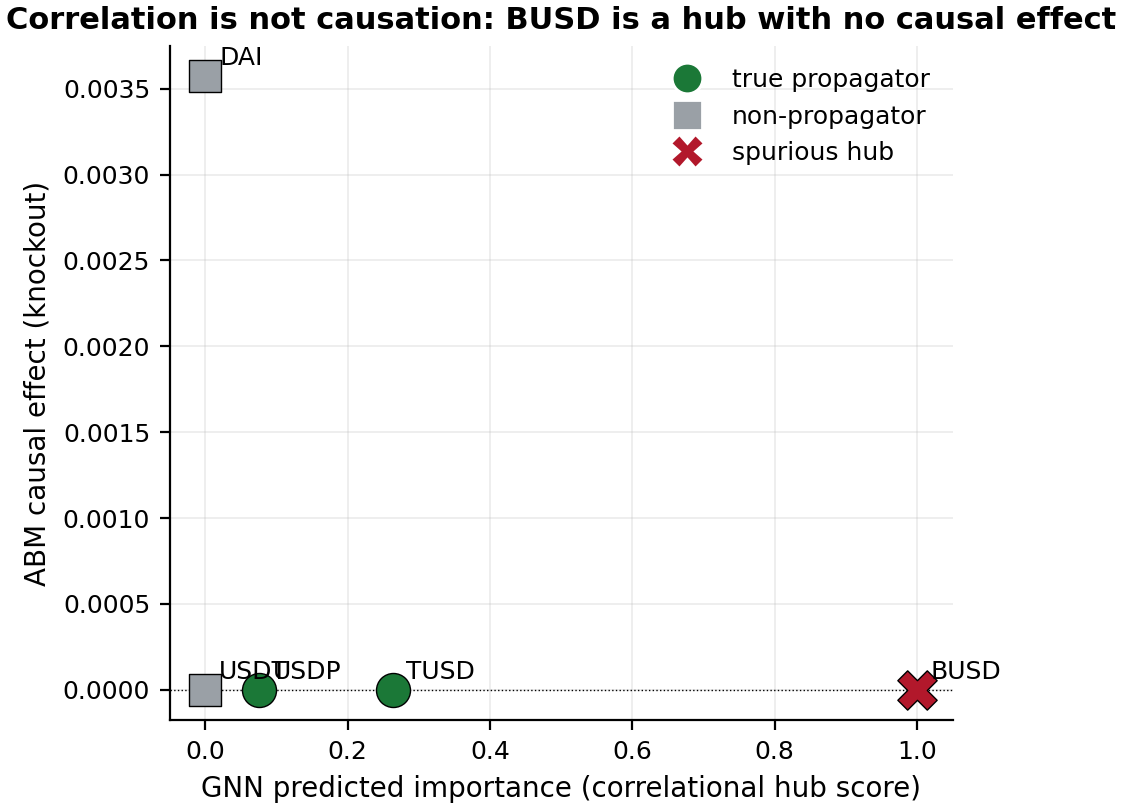
\includegraphics[width=\columnwidth]{figures/01_causal_join.png}
\caption{Correlation versus causation. The predictor's \#1 hub (BUSD, red $\times$) has causal effect
$\approx 0$; the venue with real causal effect (the relay DAI) was not flagged as a hub.}
\label{fig:join}
\end{figure}

\paragraph{What each moment buys us.} The four calibration moments are not arbitrary; each pins down a
different aspect of the dynamics that the counterfactual depends on. The \emph{contagion magnitude}
fixes the overall gain, so that a knockout's percentage reduction is meaningful. The \emph{half-life}
fixes the recovery rate $\kappa$, which determines how long a protected node's absence is felt. The
\emph{baseline volatility} fixes the noise floor, so that a causal effect can be distinguished from
chance. And the \emph{cross-venue correlation} fixes the panic channel $\pi$, which governs how much
of the co-movement is common-factor rather than direct transmission---exactly the distinction at the
heart of the BUSD result. Matching all four is what makes the knockout trustworthy.

\section{Why BUSD is spurious: the balance sheet}\label{sec:exposure}
A careful reader will object that our network $W$ was \emph{estimated} from the same prices the
predictor used, so perhaps the whole exercise is circular. We answer by rebuilding $W$ from a source
that has nothing to do with prices: \emph{documented reserve holdings}. A depeg in coin $j$ can
mechanically drag down coin $i$ only if $i$ holds $j$ as part of its backing. During the SVB window,
public disclosures show DAI held roughly 50\% USDC and FRAX roughly 90\% USDC, while BUSD, TUSD, USDP,
and USDT held no other stablecoin---and, decisively, \emph{no stablecoin held BUSD as backing}.

Under this balance-sheet network the model still calibrates to all four moments, and BUSD's
``out-exposure''---the total of other coins' reserves backed by it---is exactly zero
(Figure~\ref{fig:exposure}). It is therefore \emph{mechanically} incapable of transmitting a depeg,
regardless of how central it looks in a correlation graph. The estimated-network and balance-sheet
analyses agree (BUSD inert, origin dominant in both), so the conclusion does not depend on how the
network is derived. This is the strongest form of the result: BUSD is spurious not as a statistical
accident but as a balance-sheet fact.

\begin{figure}[t]
\centering
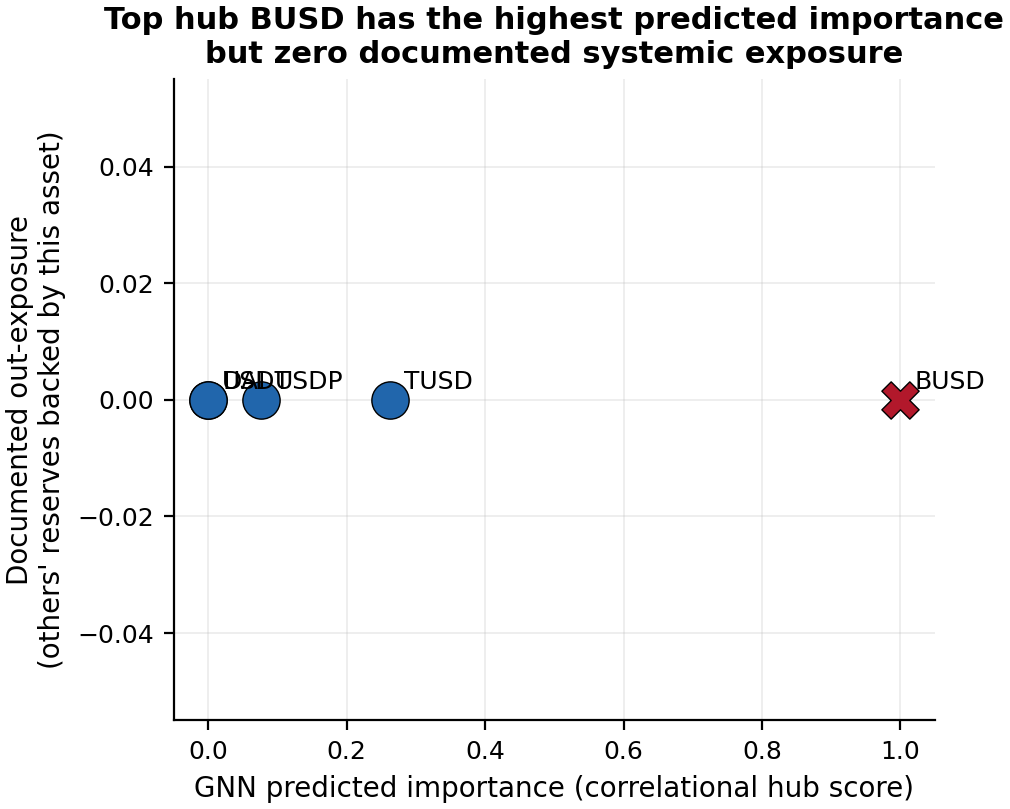
\includegraphics[width=\columnwidth]{figures/02_exposure.png}
\caption{The predictor's top hub (BUSD) has the highest correlational importance but \emph{zero}
documented systemic exposure: no stablecoin's peg depends on it.}
\label{fig:exposure}
\end{figure}

\section{Robustness}\label{sec:robust}
We subject the headline to four independent stress tests.

\paragraph{(1) Calibration uncertainty.} The calibration is not exact, so we perturb the model's
parameters and network by $\pm30\%$ over 60 random draws and re-run the knockout. USDC is the top
causal venue in $100\%$ of draws and BUSD stays causally inert in $100\%$ (Figure~\ref{fig:robust}).
The conclusion is not an artifact of one lucky calibration.

\paragraph{(2) Strategic agents.} To address the worry that our model is too mechanical, we add two
behavioural agents (Figure~\ref{fig:twoagent}). An \emph{adaptive redeemer} accelerates redemptions
as a coin falls, amplifying runs; a \emph{capital-capped arbitrageur} buys depegged coins to restore
the peg but runs out of capital in a large crisis (the classic ``limits to arbitrage''). The redeemer
amplifies contagion $7.7\times$ and the arbitrageur damps it, yet across all four agent configurations
USDC remains the top causal venue and BUSD remains inert---so the causal conclusion is not a
static-model artifact (a Lucas-critique check). Interestingly, the best \emph{intervention} changes:
a circuit breaker, mediocre with passive agents, becomes the most effective tool once runs are
self-reinforcing (cutting $95\%$ rather than $63\%$), because it directly interrupts the feedback
loop. A static analysis would have mis-ranked the policies---an independently useful finding.

\begin{figure}[t]
\centering
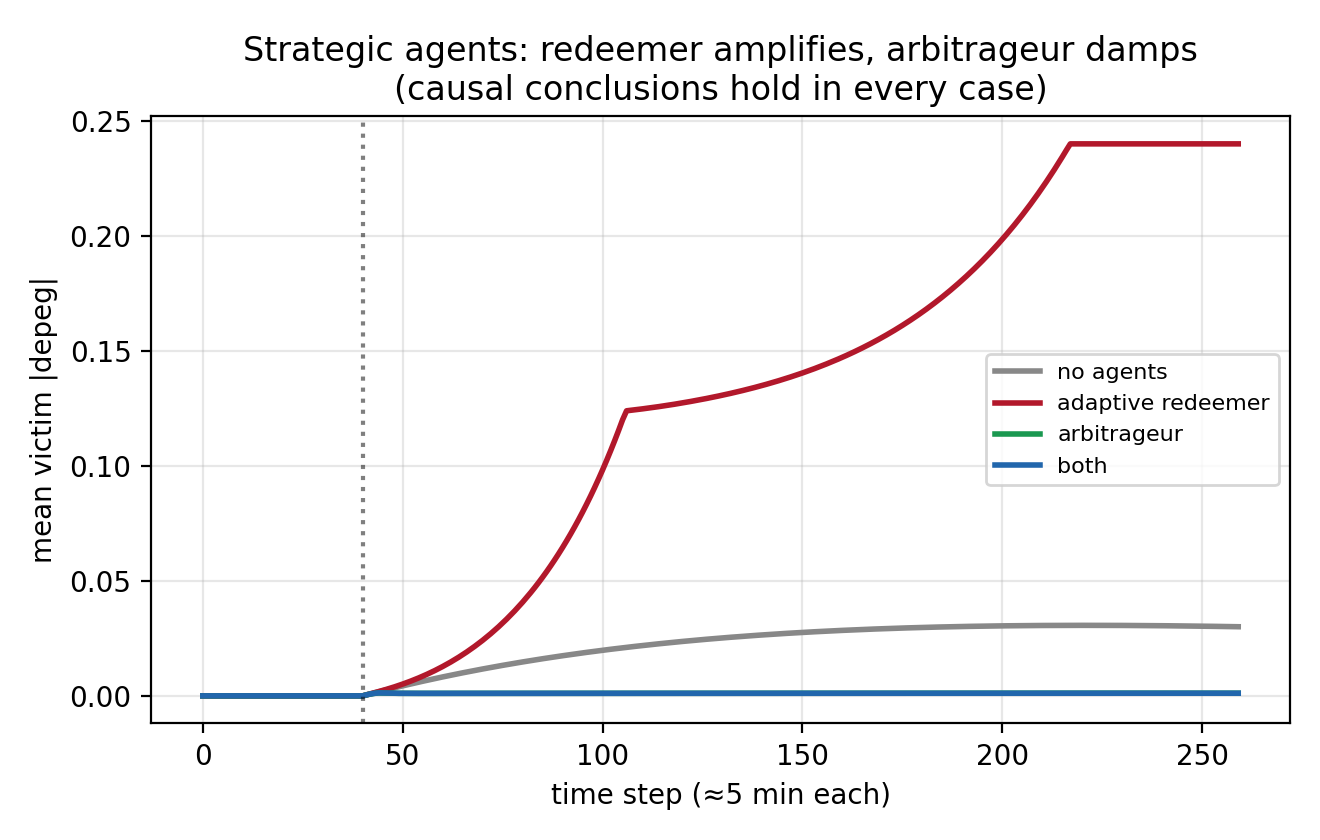
\includegraphics[width=\columnwidth]{figures/08_two_agent.png}
\caption{Strategic two-agent market. Mean victim depeg over time: the adaptive redeemer amplifies the
crisis, the capital-capped arbitrageur damps it. In every configuration the causal ranking (USDC
top, BUSD inert) is unchanged.}
\label{fig:twoagent}
\end{figure}

\paragraph{(3) Network derivation.} As shown in \S\ref{sec:exposure}, replacing the estimated network
with the documented balance-sheet network leaves the marquee result unchanged.

\paragraph{(4) Placebo / negative control.} Finally we test the method itself on synthetic data with
a \emph{known} answer. We plant a true transmission chain plus an isolated ``co-mover'' that moves
with everyone (via the panic factor) but transmits to no one. The knockout correctly assigns large
causal effect to the true transmitters and \emph{exactly zero} to the planted co-mover---a distinction
that ordinary correlation centrality cannot make (Figure~\ref{fig:placebo}). The method recovers
ground truth, so the real-data refutation reflects a property of the method, not wishful thinking.

\begin{figure}[t]
\centering
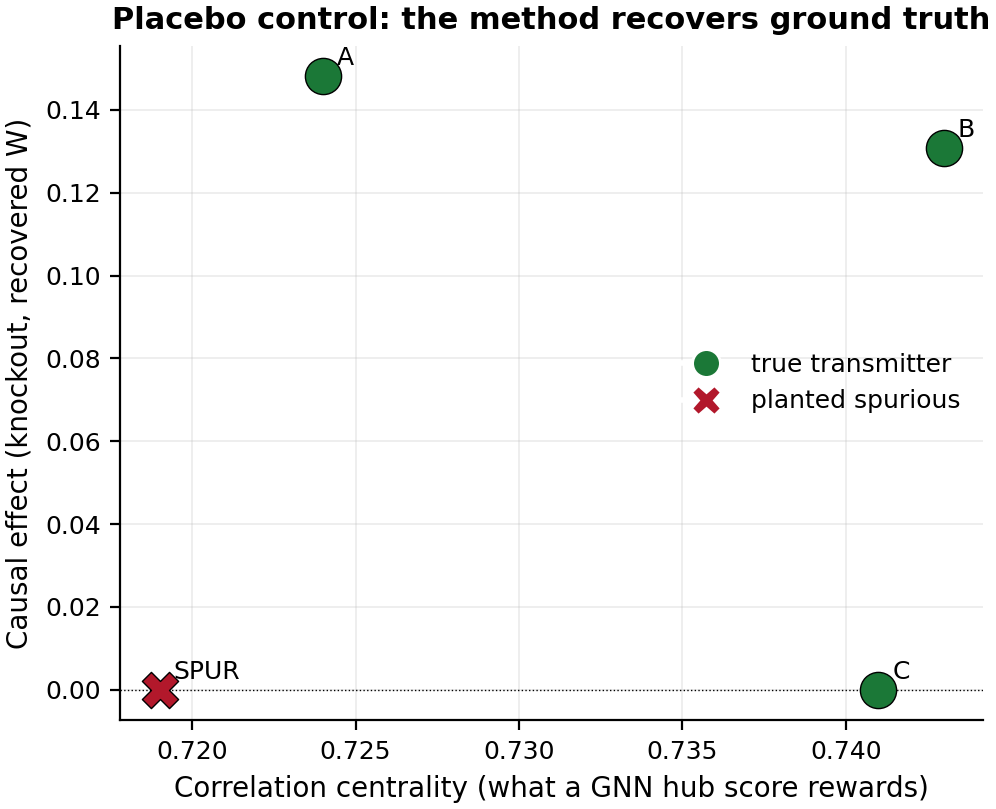
\includegraphics[width=\columnwidth]{figures/03_placebo.png}
\caption{Placebo control on synthetic data. A planted spurious co-mover (SPUR) is correlationally
central but causally inert; the knockout recovers the true transmitters.}
\label{fig:placebo}
\end{figure}

\begin{figure}[t]
\centering
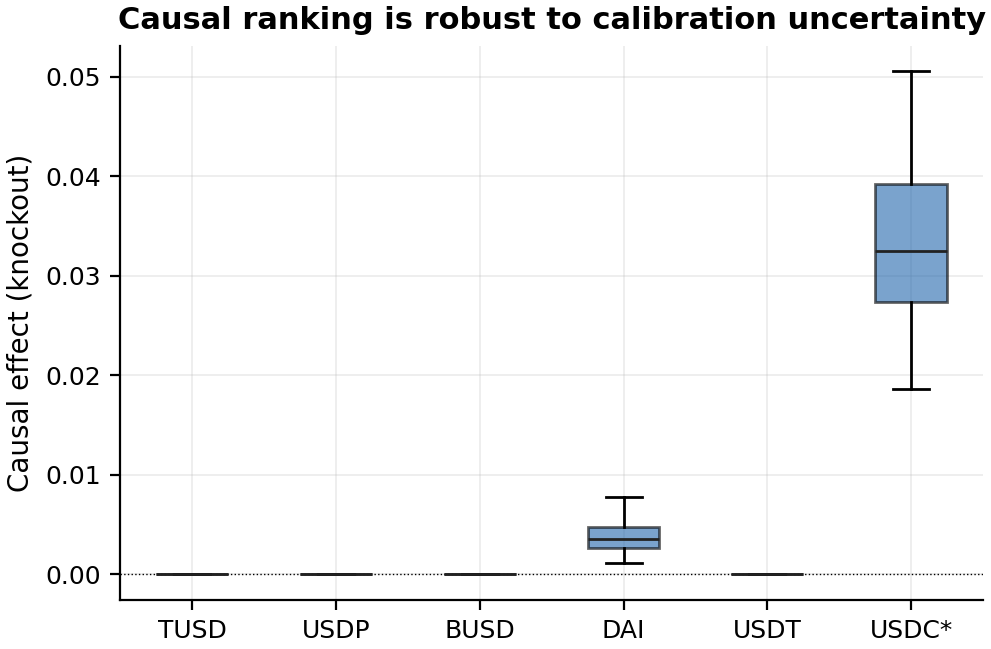
\includegraphics[width=\columnwidth]{figures/05_robustness.png}
\caption{Causal effect per venue under $\pm30\%$ calibration uncertainty (60 draws): the origin
(USDC) dominates and BUSD is pinned at zero across draws.}
\label{fig:robust}
\end{figure}

\paragraph{Does it generalize across crises?} Across the crises we can analyze
(Figure~\ref{fig:multi}), the predictor's top hub \emph{is} the causal driver in one (the Terra
collapse) but \emph{is not} in two others, so a correlational ranking is unreliable---sometimes right,
sometimes badly wrong---which is precisely why the causal test is needed. Encouragingly, a venue's
documented out-exposure, which is known \emph{before} any crisis and needs no price data, ranks
causal importance better than the learned correlational score, and the predictor's top hub is a
structurally non-transmitting (zero-exposure) venue in three of five episodes.

\begin{figure*}[t]
\centering
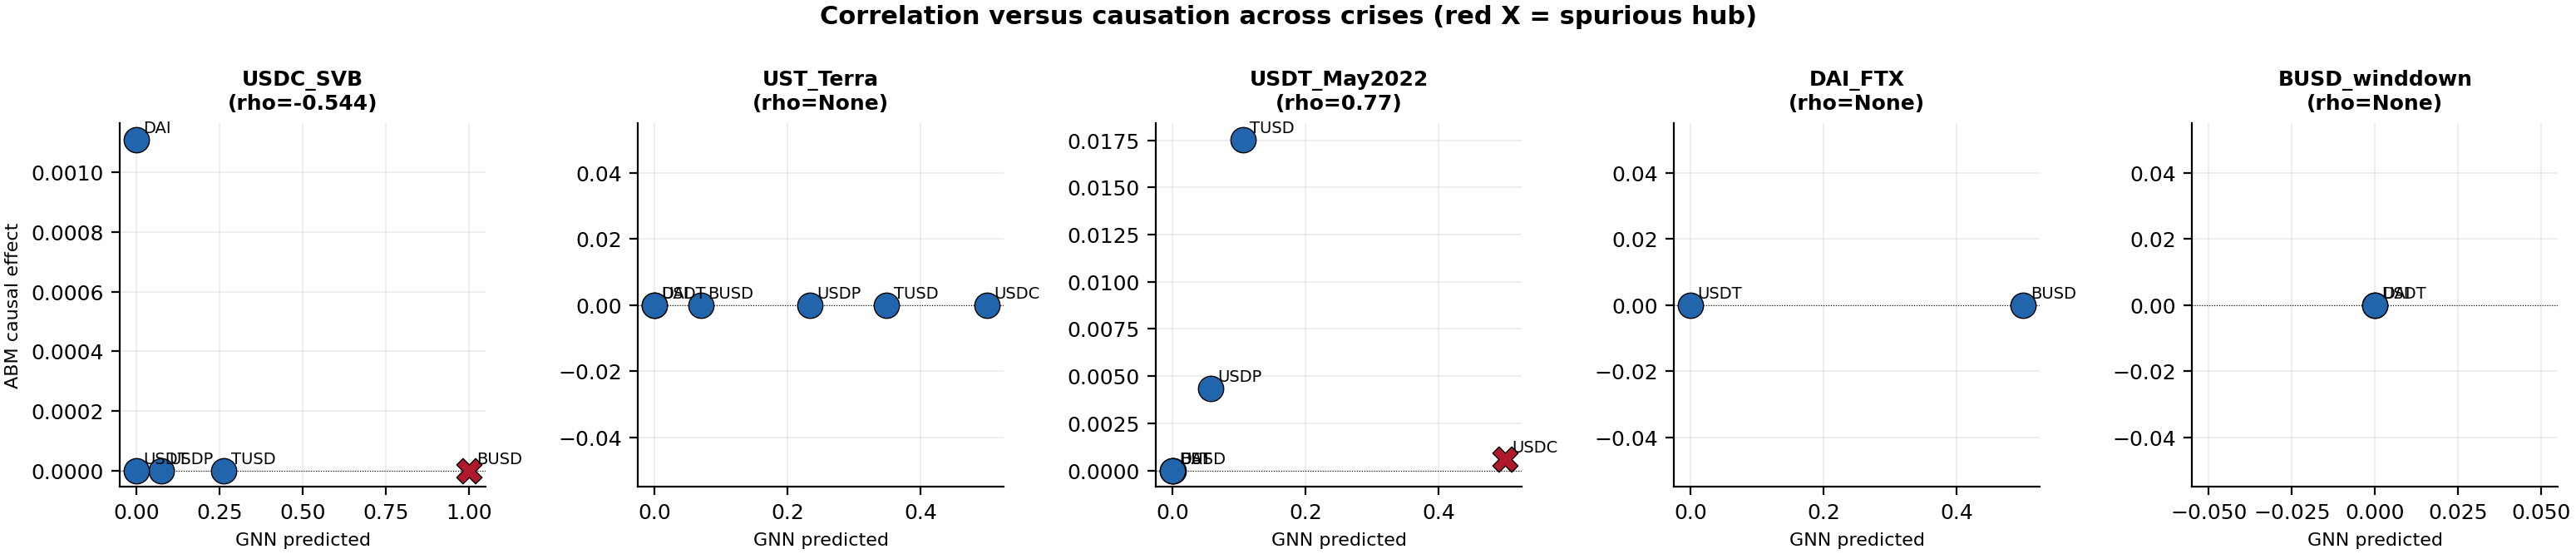
\includegraphics[width=\textwidth]{figures/06_multi_episode.png}
\caption{Correlation versus causation across crises. A red $\times$ marks a spurious hub (high
predicted importance, near-zero causal effect).}
\label{fig:multi}
\end{figure*}

\begin{table}[t]
\caption{Generalization across crises. The GNN's top hub matches the causal driver in one episode but
diverges---with a spurious, structurally non-transmitting hub---in the others.}
\label{tab:multi}
\small
\begin{tabular}{llll}
\toprule
Episode & GNN top hub & ABM causal top & spurious? \\
\midrule
USDC / SVB & BUSD & DAI & yes (BUSD) \\
UST / Terra & USDC & USDC & no \\
USDT (May) & USDC & TUSD & yes \\
\bottomrule
\end{tabular}
\end{table}

\begin{table}[t]
\caption{Two-agent robustness. The arbitrageur damps the crisis and the redeemer amplifies it, yet
the origin is the top causal venue and BUSD is inert in every configuration.}
\label{tab:twoagent}
\small
\begin{tabular}{lrcc}
\toprule
agents & baseline contagion & USDC top-causal & BUSD inert \\
\midrule
none & 0.031 & \checkmark & \checkmark \\
redeemer only & 0.240 & \checkmark & \checkmark \\
arbitrageur only & 0.0014 & \checkmark & \checkmark \\
both & 0.0014 & \checkmark & \checkmark \\
\bottomrule
\end{tabular}
\end{table}

\section{Policy: acting on causation pays}\label{sec:policy}
\paragraph{The four intervention levers.} We model the policy tools a stablecoin supervisor actually
has, each as a modification of Eq.~\eqref{eq:model}. \emph{Targeted protection / backstop}: hold a
chosen venue at its peg ($d_X\!\equiv\!0$), as in the knockout. \emph{Reserve strengthening}: raise a
venue's recovery speed $\kappa_X$ (a better-capitalised reserve mean-reverts faster).
\emph{Circuit breaker}: cap $|d_i|$ at a threshold (a trading halt that stops the depeg deepening).
\emph{Redemption gating}: reduce the global transmission gain $c$ (slowing redemptions throttles the
channel through which stress flows). Each lever has an intensity, and we sweep them.

We close with the practical payoff. In the model, protecting USDC removes $100\%$ of the contagion;
strengthening its reserves twentyfold removes $89\%$; a circuit breaker removes $85\%$; and gating
redemptions removes $100\%$. Protecting or strengthening BUSD removes \emph{nothing}, at any
intensity. The welfare decomposition (Figure~\ref{fig:welfare}) makes the distributional picture
concrete: it shows which venue bears how much loss under each policy. Protecting BUSD leaves the loss
matrix \emph{identical} to no intervention---every victim loses exactly as much---whereas protecting
USDC zeroes the entire column.

\begin{figure}[t]
\centering
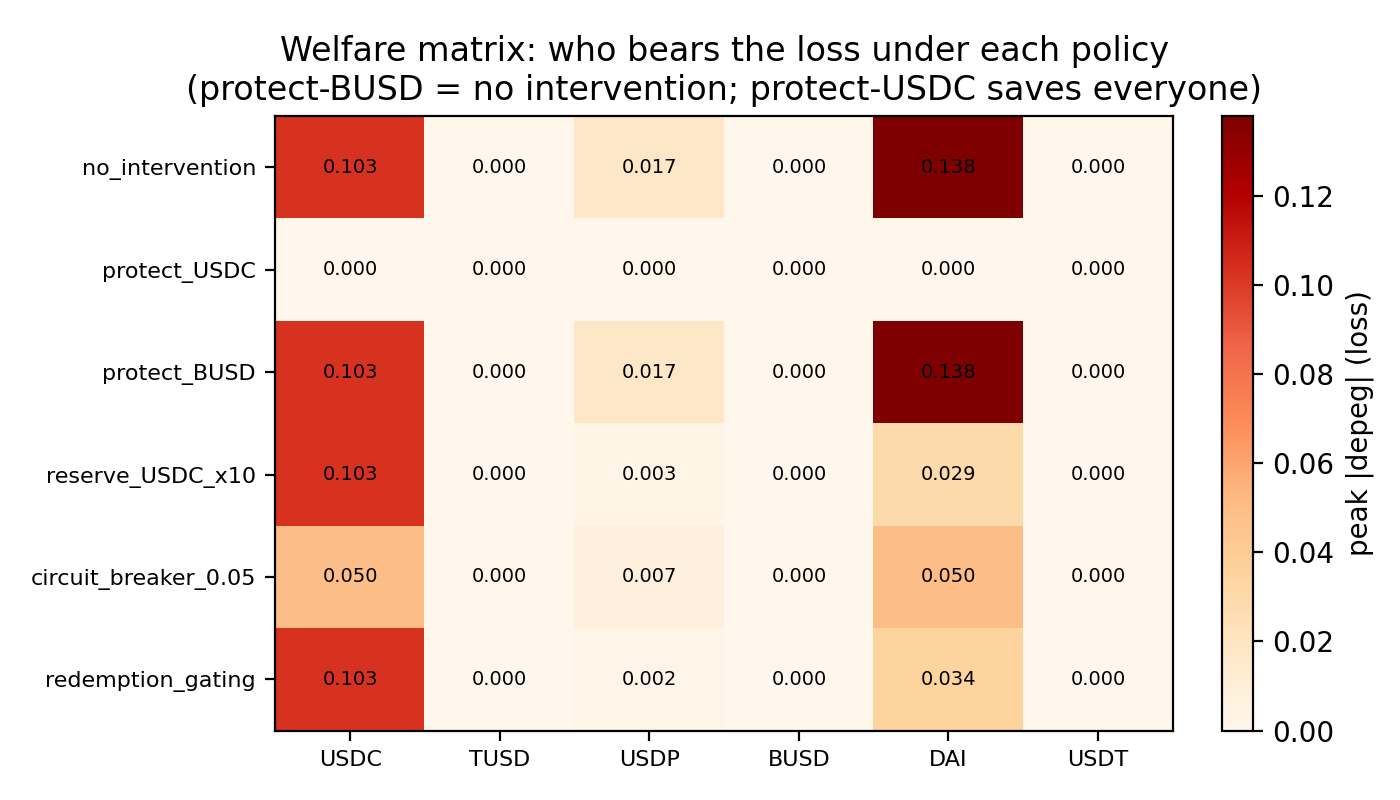
\includegraphics[width=\columnwidth]{figures/09_welfare.png}
\caption{Welfare matrix: peak depeg (loss) borne by each venue under each policy. Protecting BUSD is
indistinguishable from doing nothing; protecting USDC spares everyone.}
\label{fig:welfare}
\end{figure}

Table~\ref{tab:interventions} reports the full sweep across intervention families and intensities.
Two structural facts stand out: every intervention applied to a \emph{causal} venue (USDC) or to the
\emph{whole system} (circuit breaker, gating) works, and every intervention applied to the
\emph{spurious} hub (BUSD) does nothing.

\begin{table}[t]
\caption{Intervention sweep: contagion reduction by family and intensity. Interventions on the causal
venue or the whole system work; those on the spurious hub (BUSD) do not.}
\label{tab:interventions}
\small
\begin{tabular}{llr}
\toprule
intervention & target / setting & reduction \\
\midrule
targeted protection & USDC (origin) & 100\% \\
targeted protection & DAI (relay) & 98\% \\
redemption gating & coupling $\to 0$ & 100\% \\
reserve strengthening & USDC, $\kappa\times20$ & 89\% \\
circuit breaker & cap $2\%$ & 85\% \\
targeted protection & \textbf{BUSD} & \textbf{0\%} \\
reserve strengthening & \textbf{BUSD}, $\kappa\times20$ & \textbf{0\%} \\
\bottomrule
\end{tabular}
\end{table}

The budget comparison is the headline (Figure~\ref{fig:interventions}): a regulator who can backstop
a single venue and chooses by the correlational hub ranking protects BUSD and achieves $0\%$
contagion reduction; choosing by the causal ranking protects USDC and achieves $100\%$.

\begin{figure*}[t]
\centering
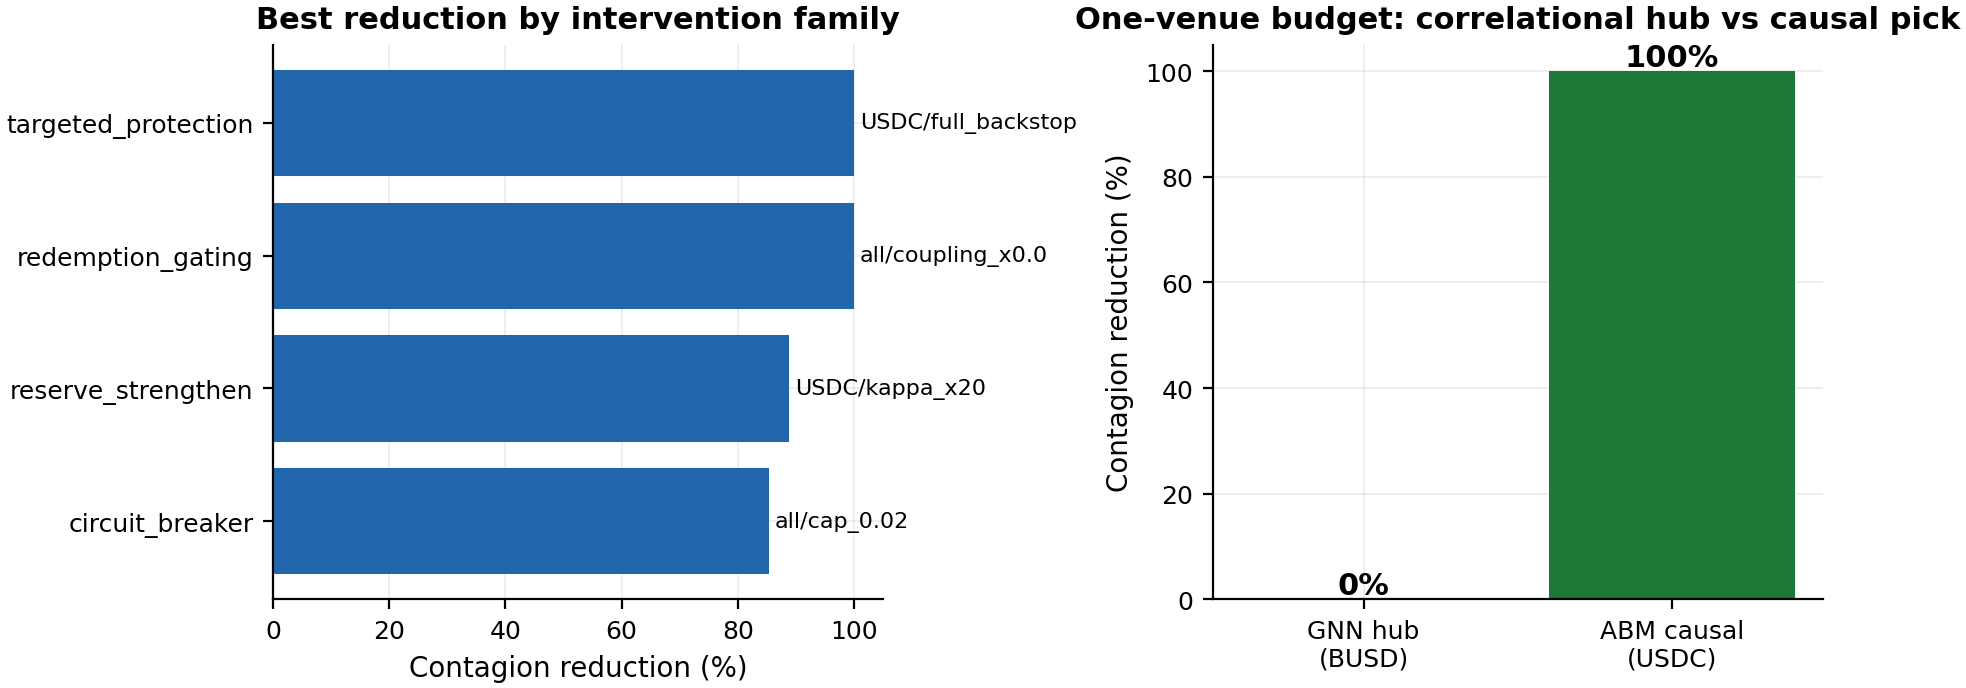
\includegraphics[width=\textwidth]{figures/04_interventions.png}
\caption{\emph{Left:} best contagion reduction by intervention family. \emph{Right:} a one-venue
budget spent on the correlational hub (BUSD) yields $0\%$; spent on the causal pick (USDC), $100\%$.}
\label{fig:interventions}
\end{figure*}

Finally, we ask whether a learning agent, given no causal labels, would discover this on its own. We
cast the problem as a one-shot contextual bandit and train a PPO~\cite{gu2024spoofability} regulator.
Its \emph{observation} is, for each venue, three purely structural features---its in-transmission,
its out-transmission, and whether it is the origin---and \emph{nothing} about which venue is causal.
Its \emph{action} is a continuous reserve-protection budget over the venues (a per-venue boost to the
recovery speed $\kappa$). Its \emph{reward} is the contagion prevented minus a cost proportional to
the budget spent, so it must learn an efficient allocation. After training, the learned policy puts
its budget on USDC and the relay DAI and \emph{none} on BUSD, achieving a $94\%$ contagion reduction
(Figure~\ref{fig:rl}). A learning agent given only the network's wiring therefore rediscovers the same
causal targets the explicit knockout identifies---and, like the knockout but unlike the correlational
ranking, never spends a cent on the spurious hub.

\begin{figure}[t]
\centering
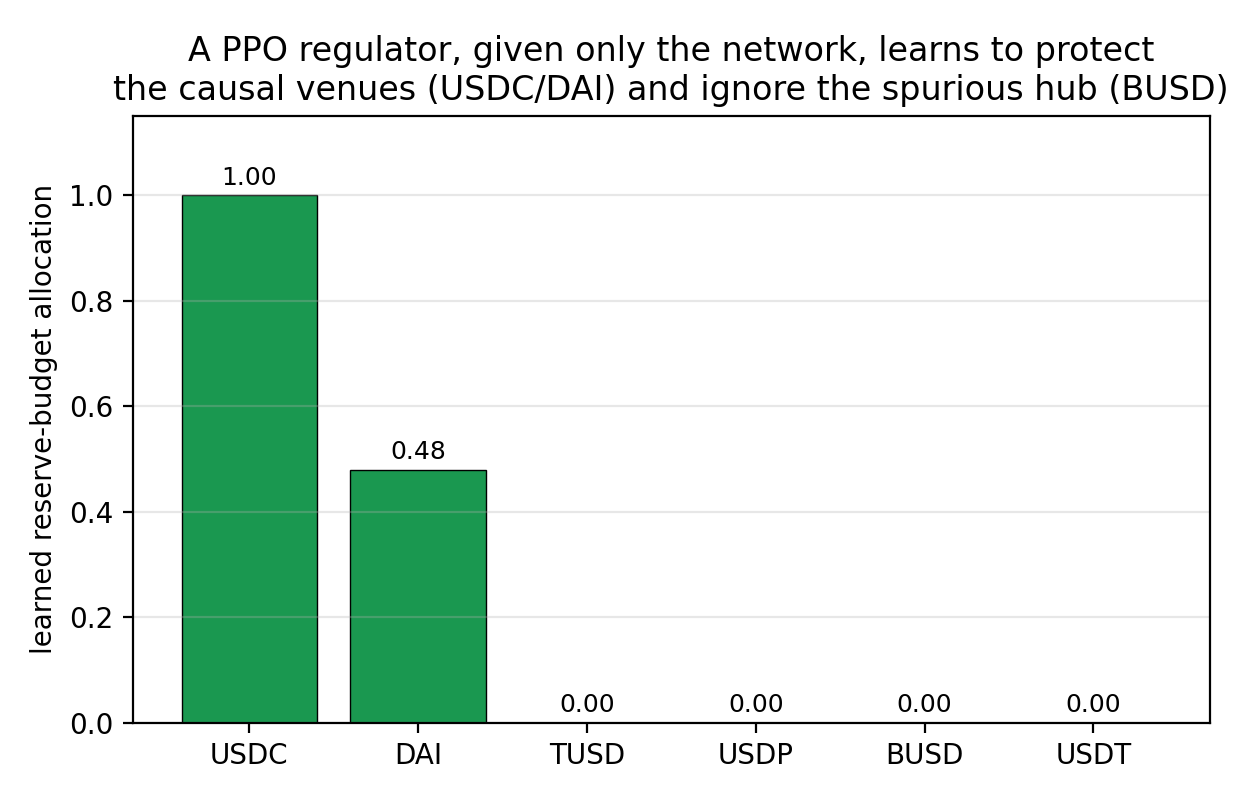
\includegraphics[width=\columnwidth]{figures/10_rl_alloc.png}
\caption{A PPO regulator, given only the network and no causal labels, learns to protect the causal
venues (USDC, DAI) and allocate nothing to the spurious hub (BUSD).}
\label{fig:rl}
\end{figure}

\section{Discussion}
\paragraph{What this means for explainable AI in finance.} Our result is a clean, quantified instance
of the spurious-correlation problem that motivates intrinsic interpretability. An attribution method
(centrality, attention) told us BUSD was \emph{the} hub; a causal test told us it transmitted nothing.
The lesson is not that the predictor is wrong---it correctly identified a venue that moves with the
crisis---but that \emph{attribution and causation are different questions}, and a high-stakes
intervention decision needs the second. Centrality answers ``what moved together?''; the knockout
answers ``what, if removed, would have changed the outcome?''---and only the latter is actionable.

\paragraph{Why BUSD looked like a hub.} BUSD was undergoing a regulatory wind-down in early 2023, so
it was being steadily redeemed and traded nervously throughout the SVB weekend. That nervous
co-movement gave it high correlation with every other stressed coin, and hence high betweenness and
high model attention. But co-movement driven by a coin's \emph{own} idiosyncratic troubles transmits
nothing to others---precisely the case the knockout is built to detect, and precisely why the balance
sheet (no one holds BUSD) is the decisive tie-breaker.

\paragraph{Practical takeaway for supervisors.} A reserve-transparency or backstop programme guided by
a correlational contagion ranking would, in this episode, have spent its capacity on a venue with no
systemic role. The same capacity directed by the causal ranking---or, equivalently here, by the
documented reserve-exposure network---would have fully contained the cascade. Where the two disagree,
the balance-sheet network is both cheaper to compute (it needs no price data) and, in our tests, the
better causal guide.

\section{Limitations and threats to validity}
Our model is a calibrated reduced form, not a fully microfounded market; two of our episodes are too
sparse to analyze causally. We address the most natural objections directly. \emph{Circularity}: the
estimated network is derived from prices, so we rebuild it from documented reserve holdings and obtain
the same answer (\S\ref{sec:exposure}). \emph{Calibration fragility}: we perturb the calibration by
$\pm30\%$ and the ranking is unchanged (\S\ref{sec:robust}). \emph{Over-mechanical agents}: we add
strategic, adaptive agents and the ranking holds (\S\ref{sec:robust}). \emph{Method self-fulfilment}:
a synthetic placebo with known ground truth shows the knockout recovers true transmitters and zeroes a
planted co-mover. The residual threat we cannot fully remove is that all causal statements are
model-based (in the structural / interventionist sense) rather than the output of a randomized
experiment, which is unavailable for historical crises; the convergence of four independent checks and
the balance-sheet confirmation is the strongest evidence the setting allows. Finally, $n=7$ episodes is
small; the load-bearing claim is therefore the single, sharply identified BUSD refutation, not a
population statistic across crises.

\section{Broader impact and regulatory considerations}
Our central message is cautionary in a way that bears directly on policy. As supervisors operationalise
the GENIUS Act and MiCA, they will need tools to decide where to focus reserve-transparency
requirements and, in a crisis, where to deploy a limited backstop. It is tempting to let a
data-driven contagion ranking make that call. We show concretely that a \emph{correlational} ranking
can send the entire budget to a venue with no systemic role: in the SVB episode it points at BUSD,
which transmitted nothing, while the venue that actually mattered (USDC, and its collateral link to
DAI) is the one a causal analysis---or simply the reserve-exposure balance sheet---identifies. The
practical recommendation is therefore conservative and, we think, robust: when the stakes are an
intervention, validate a contagion ranking against a causal counterfactual, and where the two
disagree, prefer the documented exposure network, which is transparent, auditable, and needs no
market data. A second consideration is that any such model could in principle be gamed---an issuer
aware that supervisory attention follows centrality might trade so as to appear peripheral; grounding
the analysis in mandatory reserve disclosures rather than in price-derived centrality is the natural
defence. We release all code so that the analysis can be audited and re-run on new disclosures.

\section{Future work}
The most valuable extension is to replace the estimated transmission network entirely with a
\emph{measured} balance-sheet network compiled from on-chain reserve disclosures and proof-of-reserve
attestations across the whole stablecoin universe. Such a network would make every causal statement
mechanical rather than inferred, and would let a supervisor compute the causal ranking continuously,
before any crisis, from public disclosures alone---our predictive-causality result already hints that
this static, documented quantity is the better guide. A second direction is to close the loop with the
companion predictor: use the causal verdict as a training signal, regularising the graph model toward
transmission structure that actually causes spread, so that its hub ranking and the causal ranking
converge. Finally, scaling from our seven historical episodes toward a continuously updated panel of
stress events would turn the single sharp BUSD refutation into a population-level study of how often,
and why, correlational hubs mislead.

\section{Conclusion}
Contagion hub rankings are correlational, and in the marquee SVB crisis the top-ranked hub causes
\emph{no} contagion---because, as the balance sheet confirms, no stablecoin's peg depended on it. A
calibrated, intervenable model supplies the causal test that centrality cannot, and the disagreement
is decisive for policy: acting on the correlational hub wastes the entire budget that the causal
target would have spent to contain the cascade. Contagion analytics intended to guide intervention
should report \emph{validated causation}, not centrality alone.

\paragraph{Reproducibility.} Every number above is produced by committed scripts; a single
\texttt{reproduce.sh} regenerates all results and figures end-to-end.

\appendix
\section{Reproducibility details}
The full causal pipeline runs from one script, after the companion predictor has exported its hub
ranking and calibration targets:
\begin{quote}\small\ttfamily
python scripts/run\_netcontagion\_join.py \\
python scripts/run\_exposure\_join.py \\
python scripts/run\_intervention\_sweep.py \\
python scripts/run\_multi\_episode\_join.py \\
python scripts/run\_robustness\_welfare.py \\
python scripts/run\_placebo\_control.py \\
python scripts/run\_adaptive\_robustness.py \\
python scripts/run\_two\_agent\_robustness.py \\
python scripts/run\_rl\_regulator.py
\end{quote}
Table~\ref{tab:params} lists the calibrated parameters for both versions of the model---the one whose
network is estimated from prices and the one whose network is the documented balance sheet. That the
two calibrate to the same moments with similar dynamics parameters, and yield the same causal verdict,
is the concordance that underpins our central claim. Per-draw robustness distributions, the full
intervention sweep, the welfare matrix, and the multi-episode results are all emitted as CSVs, and the
causal knockout, the exposure network, and the placebo control are unit-tested.

\begin{table}[t]
\caption{Calibrated parameters for the two model versions. Both reproduce all four moments; both put
the origin first and BUSD at zero.}
\label{tab:params}
\small
\begin{tabular}{lrr}
\toprule
parameter & estimated $W$ & documented $W$ \\
\midrule
transmission gain $c$ & 0.022 & 0.029 \\
recovery $\kappa$ (half-life 116) & 0.006 & 0.006 \\
panic $\pi$ & 0.0028 & 0.0045 \\
shock $s$ & 0.103 & 0.119 \\
\midrule
USDC causal rank & 1st & 1st \\
BUSD causal effect & 0 & 0 \\
\bottomrule
\end{tabular}
\end{table}

\bibliographystyle{ACM-Reference-Format}
\bibliography{references}

\end{document}
